\section{\lr{tokenization}}
در این قسمت مدل
\lr{SentencePiece}
با اندازه واژگان
33،
 400،
  2000،
   10000 
و
 27524
و در حالت 
\lr{\textit{model\_type = word}}
آموزش می بیند. در هر دور از آموزش $\frac{1}{5}$ از کل داده برای ارزیابی کنار گذاشته می شود تا درصد توکن
\lr{\texttt{<unk>}}
روی آن محاسبه شود. درصد توکن 
\lr{\texttt{<unk>}}
به ازای هر اندازه کلمات در شکل
\ref{fig21}
آورده شده است. همان طور که پیداست هر چه تعداد کلمات
tokenizer
کمتر باشد تعداد توکن های ناشناخته نیز بیشتر است. اما با بیشتر کردن تعداد کلماتی که 
tokenizer
می تواند تشخیص دهد، تعداد وقوع توکن
\lr{\texttt{<unk>}}
نیز کاهش می یابد.


 \begin{figure}[H]
	\centering
	
	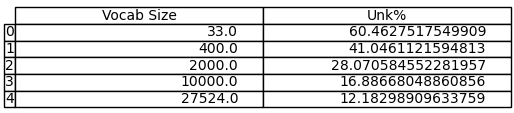
\includegraphics[width=1\textwidth,height=1\textheight,keepaspectratio]{../reports/tokenization/unk_percent}
	\caption{درصد توکن 
		\lr{\texttt{<unk>}}
		به ازای تعداد کلمات متفاوت}
	\label{fig21}
	
\end{figure}

برای مدل نهایی، تعداد کلمات 10000 انتخاب شده است. چرا که کمترین درصد توکن
\lr{\texttt{<unk>}}
را دارد و به نسبت اندازه مناسبی دارد(مدل bert 
30 هزار توکن دارد \cite{Ref4}).